%! Author = louis
%! Date = 28-10-22

\subsection{Aspects technologique}\label{subsec:aspects-technologique}
Le projet ayant comme contrainte principale d'être disponible sur toutes les plateformes majeures, une base web me paraît évidente.
Pourtant, le web implique aussi la limitation principale qu'est le besoin de connexion permanente au serveur.\\

Pour remédier à ce problème, une PWA (Application Web Progressive) nous permettrait de bénéficier des avantages du web,
tout en permettant aux utilisateurs de conserver une version locale de l'application.
De plus, une PWA permet d'être installée comme une application native Android ou iOS pour les plateformes mobiles, ce qui facilite l'accès.\
Cependant, les PWA augmentent aussi énormément la complexité du projet et limitent le développeur dans son choix d'outils.
La première version de l'application sera donc un site web responsive qui pourrait éventuellement être transformé en PWA par la suite.

Il ne faut cependant pas perdre de vue le second objectif de cette application qu'est la possibilité de la déployer simplement.

Toute application web nécessite plusieurs composants:
\begin{itemize}
    \item Une interface utilisateur
    \subitem un gestionnaire de données
    \subitem un gestionnaire de requêtes
    \subitem une libraire de composant graphique
    \item Une Couche de calculs applicatifs et de persistance de données
    \subitem Une Base de Donnée
    \subitem Un ORM
    \subitem Une API définie
%    \subitem Un système de matching pour le covoiturage
%    \subitem Un système de création de trajet pour le covoiturage
    \subitem Un système de matching pour les dettes
    \subitem Un système d'équilibrage des dépenses entre les utilisateurs
\end{itemize}

\paragraph{TypeScript}
Avant de regarder quels outils utiliser pour les différents composants, je pense qu'il est important de choisir un langage de programmation.\\

Pour ce projet, j'ai décidé d'utiliser le même langage pour les 2 composants majeurs que sont le front-end et le back-end.
Plusieurs choix s'offraient alors à moi, JavaScript, Kotlin, TypeScript ou n'importe quel langage compilable en web assembly.\\

JavaScript n'était pas vraiment un bon choix vu qu'il ne propose pas de typage, ce qui rend le code moins prédictible et robuste.\\

Kotlin est un bon candidat, il offre un typage statique, mais propose de l'inférence de type, peut être transpilé vers du JavaScript ou du web assembly,
les outils de développement pour Kotlin sont aussi très bons, mais la documentation pour une utilisation web est plutôt pauvre, comparée aux autres options.\\\\

TypeScript a quant à lui tous les avantages de Kotlin, grâce au typage fort, et profite aussi de la documentation et des outils JavaScript grâce à sa nature de superset.
Lorsque l'on développe un produit web, surtout pour un développeur full-stack, TypeScript est l'idéal.\\
Ses outils, l'environnement JavaScript, la sécurité des types et du null, la documentation, sont toutes de bonnes raisons d'utiliser TypeScript.
Pour toutes ces raisons, TypeScript est le langage idéal pour le développement Web.

\subsubsection{Front-end}\label{subsec:front-end}
Pour ce qui est de l'interface utilisateur ( le front-end ) j'ai décidé d'utiliser Angular car ce framework utilise TypeScript nativement tout en supportant aussi les PWA\@.
Angular étant un framework orienté, il m'oblige aussi à suivre une architecture propre qui permet de rendre independents les différents composants du projet .

\paragraph{Gestion des données}
Pour conserver les données hors ligne et facilité l'accès à des données à jour lors d'une connexion j'ai décidé d'utiliser NgRx.
Ce dernier est un framework de gestion de données qui simplifie l'accès et le caching de données

\paragraph{Gestionnaire des requêtes}
Lorsque l'on veut interagir avec une API graphql il est préférable d'utiliser un client.\\\\

Il existe une multitude de clients GraphQl mais le plus populaire et le mieux documenté reste Apollo.
De plus il existe un wrapper pour le client Apollo qui l'intègre dans Angular nommé Apollo Angular.
Je vais donc utiliser cette librairie pour récupérer mes données au pres de mon serveur .

\paragraph{librairie CSS}
Utiliser une librairie de composants permet de simplifier la création de l'interface grâce à des blocks de construction appelé composants\@.
Angular permet d'utiliser des librairies de composants avec leur propre logique, structure, et CSS\@.
Ces librairies fournissent aussi un ensemble de classe CSS pour rendre nos propres composants jolis.\\
De plus, elles permettent de rendre notre application responsive sans devoir y penser pour chaque composant.
Il existe plusieurs librairies majeures, les principales sont:
\begin{itemize}
    \item Angular Material
    \item PrimeNg
    \item NgBootstrap
\end{itemize}
Angular Material est la librairie officielle, elle est d'origine Google,
offre beaucoup de composants différents en plus de plusieurs composants de layout qui permettent de d'organiser d'autres composants sur la page.\\\\

PrimeNg offre aussi un grand nombre de composants, mais n'offre pas de layout par contre,
PrimeNg permet d'utiliser un autre thème que Material.\\\\
NgBootstrap est un simple wrapper pour Bootstrap css et propose tous les composants de bootstrap.
Vu que mon objectif final serait de créer une PWA qui sera installable sur Android,
utiliser un thème similaire à ceux des applications Google intégrera mieux l'application.

\subsubsection{Back-end}\label{subsubsec:back-end}
Le serveur back-end doit être capable de mettre à disposition les données nécessaires au fonctionnement de l'application.
Cependant, le back-end sera aussi responsable des calculs d'équilibrage des dépenses, des matching de covoiturage et des trajets.\\\\

Connaissant déjà Express.js et Spring (Kotlin) je me suis naturellement tourné vers ces derniers, néanmoins je désirais utiliser du TypeScript pour ce projet.
Express.js est compatible avec TypeScript mais Spring ne l'est pas.
Express.js est leger, minimaliste et propose une bonne documentation,
Spring est généraliste propose des outils de génération de code et utilise un système d'injection de dépendance.\\

Ce qu'il me fallait était une hybride entre Spring et Express.js.
Après quelque recherches, j'ai trouvé un framework appelé Nest.js, ce dernier supporte nativement TypeScript, propose une documentation excellente,
propose un CLI permettant de générer du code boiler-plate, reste simple et leger, utilise de l'injection de dépendance et est très utilisé et apprécié par d'autres développeurs.
J'ai donc décidé d'utiliser Nest.Js pour ce projet.

\paragraph{ORM}
Nest.Js (que je vais appeler Nest à partir de maintenant) n'est pas un framework batteries included comme le sont Spring ou Laravel,
Il m'a alors fallu choisir aussi un ORM pour interfacer avec ma base de données.
Dans la Documentation de Nest, il y a des exemples de configuration avec les ORM les plus utilisés avec Nest et TypeScrip.
Ces derniers sont Sequelize, TypeOrm ainsi que Prisma.
Ayant eu une experience avec Sequelize plutôt mauvaise lors de mon projet de dev3, j'ai décidé de regarder du côté de prisma.\\

Prisma est une ORM un peu particulière dans le sens où il propose d'utiliser un schema prisma pour définir ses entités au lieu d'utiliser du code TypeScript.
Cella me paraissait une très bonne chose vu que prisma générait alors lui-même les différents DTO nécessaires.
Il s'est cependant avéré qu'à l'utilisation prisma n'est pas l'idéale surtout lorsque l'on désire le coupler à une API graphQl.\\

À cause de son schema particulier, je devais définir le forma de mes entités à 2 endroits et tout de même créer manuellement mes DTO\@.
Sans compter que les opérations de CRUD dans les entités étaient rendues très complexe dû aux liens entre elles et que Prisma ne permet pas d'utiliser des identifiants.\\\\
J'ai donc décidé de jeter un oeil à TypeOrm, celui-ci propose de définir les entités via des annotations TypeScript.
Ce qui me permet d'utiliser une seule classe pour définir mon entité d'ORM et de graphQl de plus TypeOrm est mieux
documenté gràce au support d'une communauté plus large.

\paragraph{L'API back end}
Il existe plusieurs types d'API très utilisées pour le Back-end, mais les plus populaires sont le REST et le SOAP\@.
SOAP est de moins en moins utilisé dû à la complexité intrinsèque du xml et à sa lourdeur.\\\\
Il nous reste alors REST qui est une bonne solution, mais nécessite pour presque chaque requête de récupérer des données qui ne seront pas toujours consommées par le client.
Avec Rest lorsque l'on récupère une entité complete tous les champs sont renvoyés.
C'est pour cela que graphQl a été crée, non seulement graphQL utilise un typage fort via un schema défini et exposé par le serveur,
mais en plus graphql permet de ne récupérer que les champs nécessaires au client grace au GQL .

\paragraph{La base de donnée}
Ma base de donnée devait me permettre 2 choses, stocker des données géographiques et faire des operations sur ces données.
Le seul choix qui s'offrait à moi compatible avec TypeOrm était Postgres avec une extension nommée POSTGIS\@.
Postgres est une base de donnée très utilisée en production, très performante et stable.

\paragraph{Structure de donnée}
Pour stocker toutes les données nécessaires au fonctionnement de l'application, il nous faut une structure de donnée cohérente.
Voici un schema\ref{fig:dbSchema} de la base de donnée et de sa structure:

%Todo: fix possitioning Shema DB and update
\begin{figure}[htbp]
    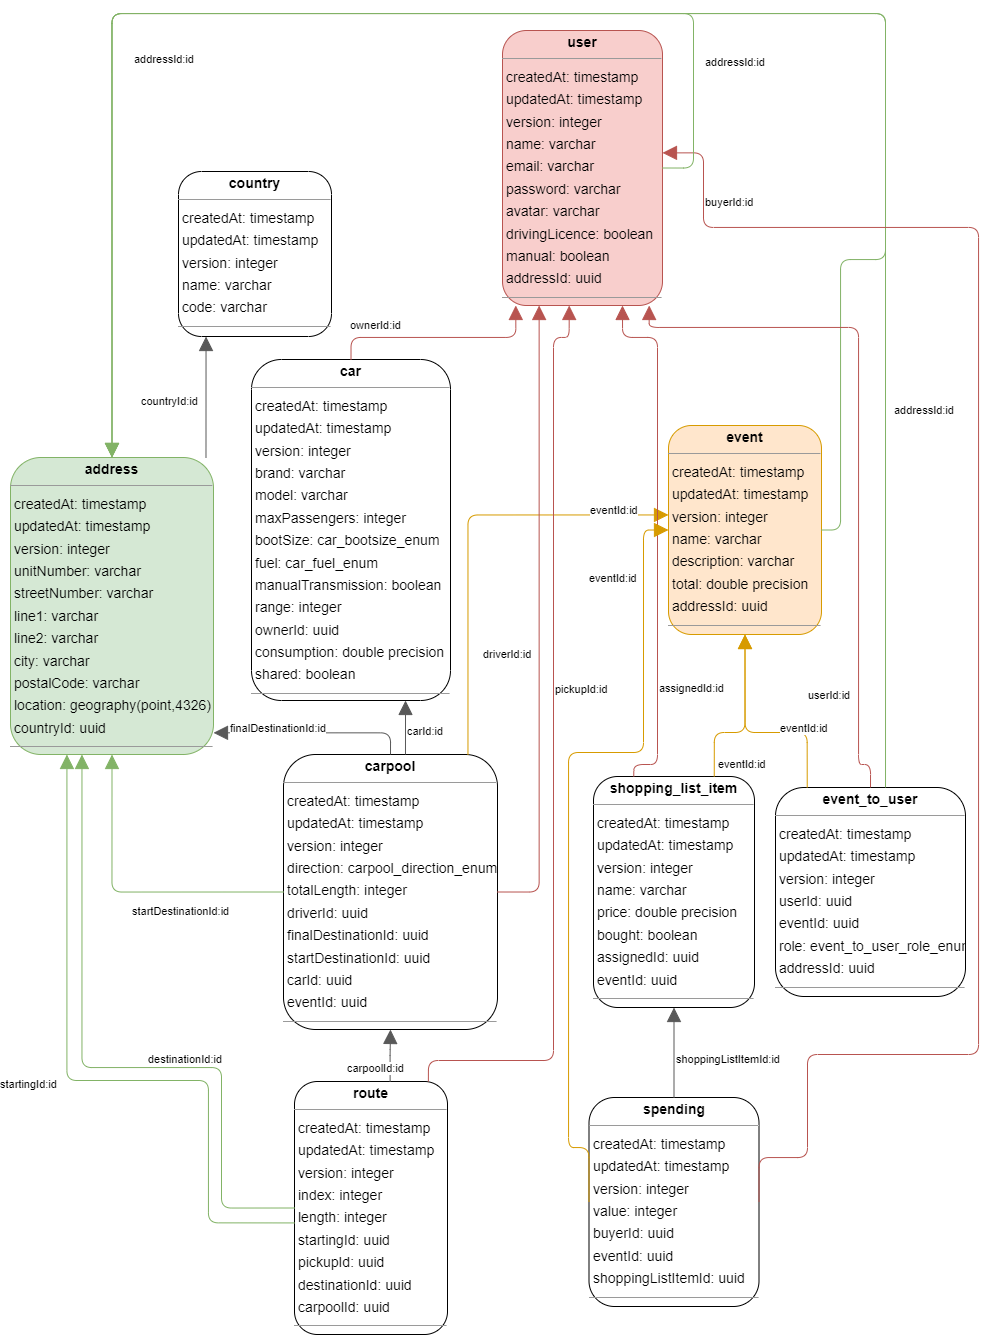
\includegraphics[width=\linewidth]{./images/dbShema}\caption{Architecture de la base de donnée}\label{fig:dbSchema}
    \centering
\end{figure}

\newpage

\subsubsection{Hébergement}\label{subsubsec:hebergement}
Afin de permettre aux utilisateurs souhaitant auto-héberger l'application, il est essentiel de fournir un environnement préconfiguré ou indépendant de l'hôte.
La meilleure solution, en l'occurrence, consiste à conteneuriser l'application.

\paragraph{Conteneurisation}
Pour mettre en conteneur l'application, diverses options sont disponibles.
Nous pourrions, par exemple, créer une image Docker englobant l'ensemble de l'application.
Cette image comprendrait à la fois la base de données, le service d'API et le serveur web hébergeant l'interface utilisateur.
Bien que cette solution soit loin d'être idéale, elle offre un avantage considérable pour l'utilisateur, en permettant la mise en place de l'application en une seule commande.\\

Cependant, cette approche ne facilite pas l'ajout de services supplémentaires, tels qu'un serveur de messagerie ou un autre type de base de données, par d'éventuels futurs développeurs.
Afin de conserver les avantages de cette solution monolithique tout en séparant les différents services (serveur web, API, base de données, etc.) dans des conteneurs distincts,
nous pourrions utiliser des outils tels que Docker Swarm, Docker Compose ou d'autres systèmes d'orchestration, tels que Kubernetes. \\

Un script Docker Compose simple semble être la meilleure option pour permettre aux utilisateurs souhaitant auto-héberger l'application de manière aisée.
Néanmoins, il serait également intéressant d'offrir la possibilité aux utilisateurs plus avancés d'héberger l'application avec une haute disponibilité.

\paragraph{Orchestration}
Afin d'assurer une haute disponibilité, il est essentiel que l'application ne présente aucun point de défaillance unique.
Par exemple, sans haute disponibilité, si le système d'exploitation du serveur subit un crash, l'ensemble de l'application serait impacté.
Pour renforcer la résilience face à ce type de problème,
nous introduirons de la redondance à tous les niveaux du système d'hébergement en utilisant un outil d'orchestration de conteneurs sur plusieurs machines.\\

Plusieurs outils d'orchestration de conteneurs pour un cluster de machines sont disponibles, mais Kubernetes se distingue par sa simplicité d'approche.
Nous mettrons donc en place un cluster Kubernetes pour héberger l'application avec une haute disponibilité.
De plus, ce cluster facilitera également la gestion des certificats TLS\@.\\

Toutefois, la mise en place d'un cluster Kubernetes ne garantit pas la portabilité de notre cluster.
Une fois établi, il demeure unique, à l'instar d'un flocon de neige.
Pour résoudre ce problème, nous ferons appel à l'infrastructure en tant que code (Infrastructure as Code - IaC).

\paragraph{Infrastructure as code}
Comment rendre notre cluster et par extension notre application déployable en une seule commande ?
J'ai opté pour l'utilisation d'Ansible afin de déployer mon cluster, indépendamment de l'état de la machine.
Ansible offre effectivement une approche agnostique qui facilite le processus de déploiement.\\

Un simple script shell aurait pu être utilisé, mais il ne serait pas agnostique par rapport à l'état de l'OS\@.
Par exemple, si une commande demande de créer le répertoire /home/foo mais qu'il existe déjà, le script shell échouerait.
En revanche, Ansible poursuivra son exécution sans problème, car pour lui, si le répertoire existe déjà, cela signifie que l'objectif est atteint.\\

\subsection{Aspect non technologique}\label{subsec:aspect-non-technologique}

\subsubsection{Tests unitaires et tests d'intégration}

Le code de l'application est testé à l'aide de tests unitaires et de tests d'intégration pour le backend.
Ces tests permettent de vérifier le bon fonctionnement des fonctionnalités individuelles et de leur intégration au sein de l'ensemble du système.

\subsubsection{Sécurité et confidentialité}

\paragraph{Sécurité}
L'application n'utilise pas HTTPS vu que cela nécessiterait des certificates SSL, cependant il est vivement conseiller d'utiliser un reverse proxy pour réaliser la terminaison SSL.\\
Néanmoins, les mots de passe sont chiffrés et salés avant d'être stockés en base de données grâce à Argon2.\\

Angular et NestJs permettent d'empêcher les attaques de type SQL injection. \\

En ce qui concerne les attaques de type DoS ou DDoS, aucune protection n'est mise en place au niveau applicatif, car il est plus simple d'implémenter cette sécurité au niveau du réseau.\\\\

\paragraph{GDPR}
En ce qui concerne le GDPR, aucune donnée récoltée n'est revendue ni redistribuée.\\

Seules les données fournies directement par les utilisateurs via les formulaires sont récoltées et utilisées uniquement dans l'application.
Ces données peuvent être supprimées définitivement avec une simple requête à l'API\@.

\subsubsection{Accessibilité}

Le site web utilise des composants HTML standards, ce qui permet à tous de l'utiliser.
De plus, grâce aux librairies CSS, le contraste est garanti, ce qui améliore l'accessibilité pour les utilisateurs ayant des problèmes de vision.

\subsubsection{Optimisation et performance}

L'application web intégrera un système de cache grâce à Apollo Angular et sera minifiée pour la mise en production.
Ces optimisations permettent d'améliorer les performances et la rapidité de l'application.

\subsubsection{Documentation}

Le projet sera documenté via le fichier README et directement dans le code.
Des noms de variables et de fonctions explicites, ainsi qu'un typage fort, assurent une solide base de documentation.
Les fonctions plus complexes nécessitant une documentation plus approfondie seront documentées avec de la Javadoc.\\

Pour ce qui est de l'API, le schéma GraphQL sert de documentation.\\

De plus un linter est mis en place pour assurer le respect des bonnes pratiques.

\subsubsection{Gestion de projet}

Focalboard a été choisi comme outil de gestion de projet.
Il est très similaire à Trello, mais il est open-source et est auto-hébergé sur mon serveur.
Cela permet de suivre l'évolution du projet et de gérer les tâches à accomplir efficacement.\\

De plus le code sera gere au moyen de repository git

\subsubsection{Modularité et évolutivité}

L'application étant construite avec Angular et NestJs, elle est très modulaire par nature.
Cela facilite son évolution et permet d'ajouter ou de modifier des fonctionnalités sans impacter l'ensemble du système.


%todo: algorithm
